%*----------- SLIDE -------------------------------------------------------------
\begin{frame}[c]{Justificativa}
    \begin{itemize}
        \item acompanhamento, monitoramento e investigação subaquático
        \item dificuldade de acesso para mergulhadores
        \item regiões de riscos para os mergulhadores
    \end{itemize}

    \begin{figure}
        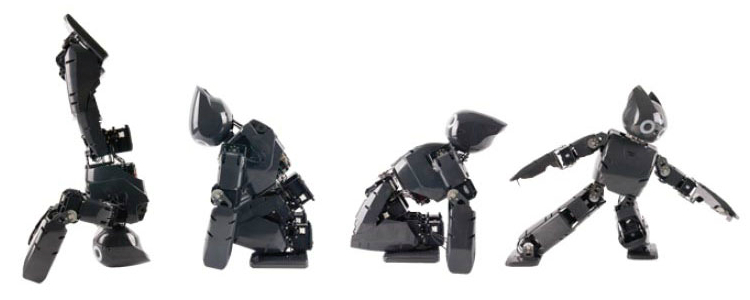
\includegraphics[trim = 0 20 0 50, clip, width=0.8\textwidth]{darwin-op-sequencia}
        %\caption{.}
    \end{figure}
%*----------- notes
    \note[item]{Notes can help you to remember important information. Turn on the notes option.}
\end{frame}
%-
%*----------- SLIDE -------------------------------------------------------------
\begin{frame}[t]{Objetivos}
    Objetivo Geral
    \newline
    Desenvolver um modelo de veículo submarino para a navegação em águas rasas.
    \newline

    Objetivos Específicos
    \begin{itemize}
        \item Realizar o estudo do estado da arte
        \item Realizar o desing da estrutura do submarino
        \item Realizae simuolações (CFD,ROS)
        \item Desenvolver o planejamento dos experimentos
        \item Desenvolver artigos científicos
    \end{itemize}
   

%*----------- notes
    \note[item]{Notes can help you to remember important information. Turn on the notes option.}
\end{frame}
%-
%*----------- SLIDE -------------------------------------------------------------
\begin{frame}[c]{Metodologia }
    %\transboxin[duration=1,direction=30]
        \begin{figure}
        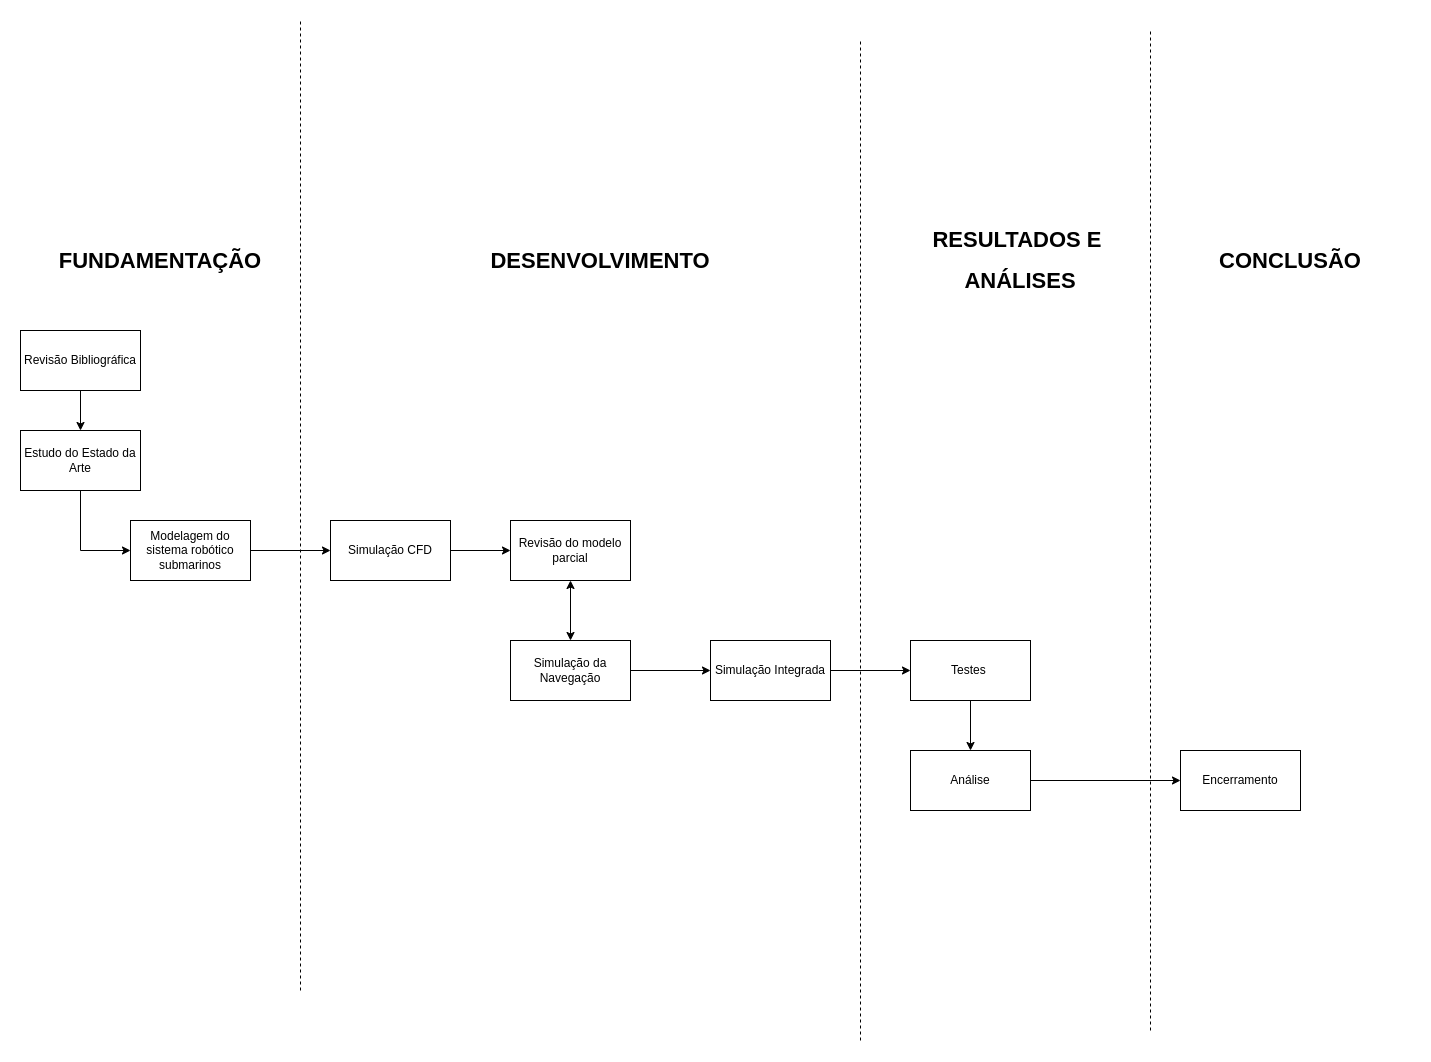
\includegraphics[width=.8\textwidth]{metodologia.png}
    \end{figure}
%*----------- notes
    \note[item]{Notes can help you to remember important information. Turn on the notes option.}
\end{frame}
%-
%*----------- SLIDE -------------------------------------------------------------
\begin{frame}[t]{O sistema robótico}
    \transboxout[duration=0.5]
    \framesubtitle{Darwin-OP}
    \begin{columns}
        \column{.1\textwidth}
        \column{.4\textwidth}
            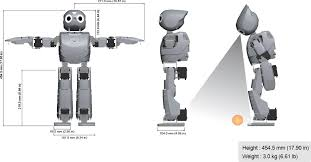
\includegraphics[width=.7\textwidth]{darwin-op}
        \column{.4\textwidth}
            \begin{enumerate}
                \item plataforma antropormórfica Darwin-OP;
                \item 20 DoF\footnote{do inglês, graus de liberdade};
                \item composto de 18 servo-motores;
                \item possui um grande gama de sensores para interação.
            \end{enumerate}
    \end{columns}
 %*----------- notes
    \note[item]{Notes can help you to remember important information. Turn on the notes option.}
\end{frame}
%-
%*----------- SLIDE -------------------------------------------------------------
\begin{frame}[c]{Darwin-OP - overview}
    %\transboxin[duration=1,direction=30]
    \centering

    \includemedia[
      width=0.7\linewidth,
      totalheight=0.39375\linewidth,
      activate=pageopen,
      passcontext, 
      addresource=./Source/movies/Darwin-OP.mp4,
      flashvars={
      source=./Source/movies/Darwin-OP.mp4
      &autoPlay=true
      &Loop=false}
      ]{\fbox{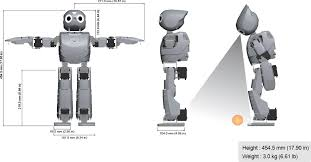
\includegraphics{darwin-op}}}{VPlayer.swf}

%*----------- notes
    \note[item]{Notes can help you to remember important information. Turn on the notes option.}
\end{frame}
%-
%*----------- SLIDE -------------------------------------------------------------
\begin{frame}[t]{O sistema robótico}
    \transboxout[duration=0.5]
    \framesubtitle{Darwin-OP}
    \begin{columns}
        \column{.1\textwidth}
        \column{.4\textwidth}
        \column{.4\textwidth}
    \end{columns}

    \begin{block}{Um bloco de destaque}
        Um exemplo de block.\\
        Oferece um certo destaque.
    \end{block}

    \begin{alertblock}{Um bloco de destaque}
        Um exemplo de alertblock.\\
        Oferece um certo destaque.
    \end{alertblock}

    \begin{exampleblock}{Um bloco de destaque}
        Um exemplo de exampleblock.
    \end{exampleblock}
 %*----------- notes
    \note[item]{Notes can help you to remember important information. Turn on the notes option.}
\end{frame}
%-
%*----------- SLIDE -------------------------------------------------------------
\begin{frame}[t]{O sistema robótico}
    \transboxout[duration=0.5]
      
    \tikzstyle{every node}=[draw=black,thick,anchor=west]
    \tikzstyle{selected}=[draw=red,fill=red!30]
    \tikzstyle{optional}=[dashed,fill=gray!50]

    \begin{tikzpicture}[%
        grow via three points={one child at (0.5,-0.7) and
        two children at (0.5,-0.7) and (0.5,-1.4)},
        edge from parent path={(\tikzparentnode.south) |- (\tikzchildnode.west)}]
        \node {texmf}
          child { node {doc}}		
          child { node {fonts}}
          child { node {source}}
          child { node [selected] {tex}
            child { node {generic}}
            child { node [optional] {latex}}
            child { node {plain}}
          }
          child [missing] {}				
          child [missing] {}				
          child [missing] {}				
          child { node {texdoc}};
      \end{tikzpicture}

 %*----------- notes
    \note[item]{Notes can help you to remember important information. Turn on the notes option.}
\end{frame}
%-
%*----------- SLIDE -------------------------------------------------------------
\begin{frame}[t]{O sistema robótico}
    \transboxout[duration=0.5]
    \framesubtitle{PlantUML}
    
    % Define block styles
    \tikzstyle{decision} = [diamond, draw, fill=blue!20, 
    text width=4.5em, text badly centered, node distance=3cm, inner sep=0pt]
    \tikzstyle{block} = [rectangle, draw, fill=blue!20, 
    text width=5em, text centered, rounded corners, minimum height=4em]
    \tikzstyle{line} = [draw, -latex']
    \tikzstyle{cloud} = [draw, ellipse,fill=red!20, node distance=3cm,
    minimum height=2em]

    \begin{tikzpicture}[node distance = 2cm, auto]
        % Place nodes
        \node [block] (init) {initialize model};
        \node [cloud, left of=init] (expert) {expert};
        \node [cloud, right of=init] (system) {system};
        \node [block, below of=init] (identify) {identify candidate models};
        \node [block, below of=identify] (evaluate) {evaluate candidate models};
        \node [block, left of=evaluate, node distance=3cm] (update) {update model};
        \node [decision, below of=evaluate] (decide) {is best candidate better?};
        \node [block, below of=decide, node distance=3cm] (stop) {stop};
        % Draw edges
        \path [line] (init) -- (identify);
        \path [line] (identify) -- (evaluate);
        \path [line] (evaluate) -- (decide);
        \path [line] (decide) -| node [near start] {yes} (update);
        \path [line] (update) |- (identify);
        \path [line] (decide) -- node {no}(stop);
        \path [line,dashed] (expert) -- (init);
        \path [line,dashed] (system) -- (init);
        \path [line,dashed] (system) |- (evaluate);
    \end{tikzpicture}

 %*----------- notes
    \note[item]{Notes can help you to remember important information. Turn on the notes option.}
\end{frame}
%-
%*----------- SLIDE -------------------------------------------------------------
\begin{frame}[t]{O sistema robótico}
    \transboxout[duration=0.5]
    \framesubtitle{PlantUML}
    
    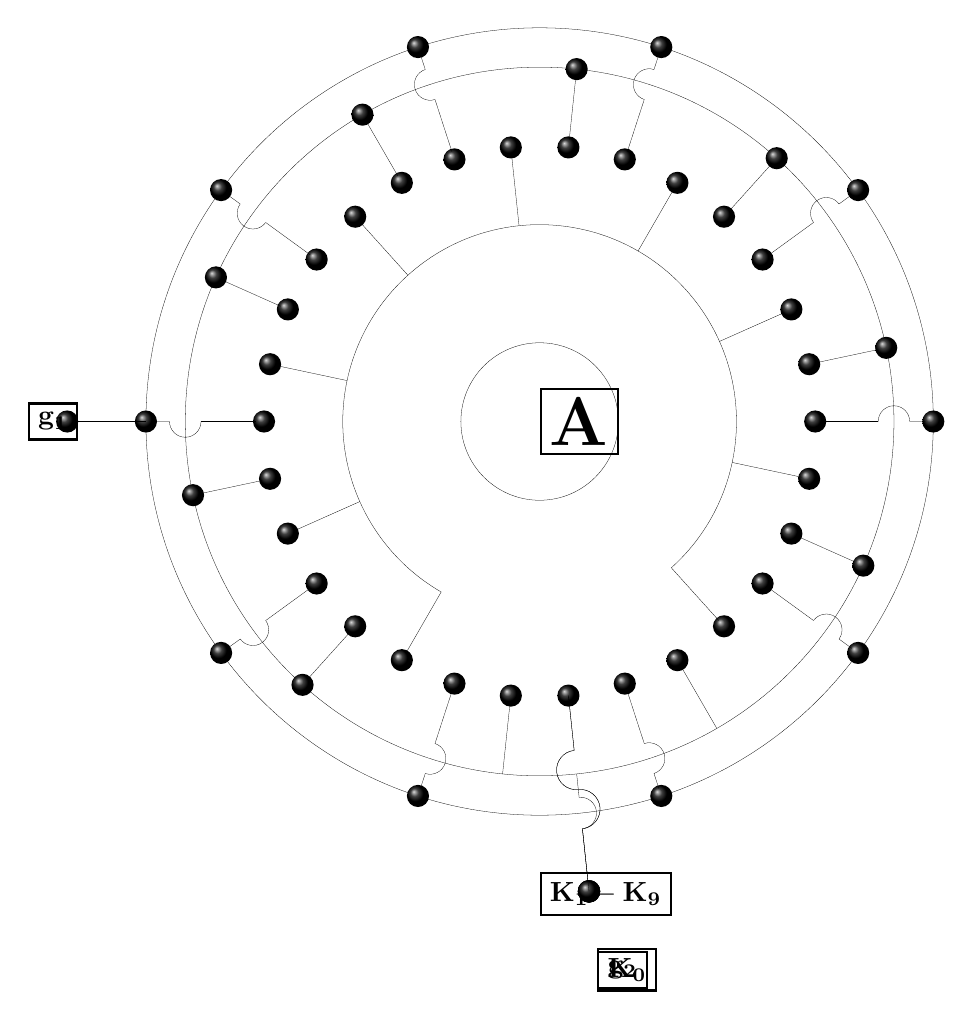
\begin{tikzpicture}[line width=0.1pt]
        \draw(0,0) circle(5cm);
        \draw(0,0) circle(1cm);
        \draw(0,0) node {\Huge$\mathbf{A}$};
        \draw(0,0) circle(4.5cm);
        \draw(-48:2.5) arc(-48:240:2.5cm);
        %% The outer nodes
        \foreach \x in {36,72,...,360}
            \shade[ball color=black](\x:5) circle(4pt);
        \foreach \nodes in {12,24,...,360}
            \shade[ball color=black](\nodes:3.5) circle(4pt);
        %%% The connecting nodes
        \foreach \angle in {-48,-12,...,240}
            \draw(\angle:2.5) --++(\angle:0.9cm);
        %%% outer interconnects
        \foreach \angle in {-24,12,...,306}
            \draw(\angle:3.6) --++(\angle:0.9cm);
        \foreach \y in {-24,12,...,240}
            \shade[ball color=black](\y:4.5cm) circle(4pt);
    
        %% outer most connections
        \foreach \angle in{-36,0,...,306}
            \draw(\angle:4.9cm) --(\angle:4.7cm) [rotate=\angle]arc(0:180:0.20cm);
        \foreach \angle in{-36,0,...,306}
            \draw(\angle:4.3cm) --(\angle:3.6cm);
        %% Outer connects and leads
        \shade[ball color=black](276:6) circle(4pt);
        \draw(276:6)circle(4pt)--(276:5.2)[rotate=276]arc(0:180:0.25cm);
        \draw(276:7)node {$\mathbf{K_0}$};
        \draw(276:4.2)[rotate=276]arc(180:360:0.25cm);
        \draw(276:4.2)--(276:3.5);
    
        %% Exploitation of circular symmetry of the required figure
    
        {[rotate=72]
            \shade[ball color=black](276:6) circle(4pt);
            \draw(276:6)circle(4pt)--(276:5.2)[rotate=276]arc(0:180:0.25cm);
            \draw(270:6)node {$\mathbf{K_1-K_9}$};
            \draw(276:4.2)[rotate=276]arc(180:360:0.25cm);%%%
            \draw(276:4.2)--(276:3.5);
        }
    
        {[rotate=-48]
            \shade[ball color=black](276:6) circle(4pt);
            \draw(276:6)circle(4pt)--(276:5.2)[rotate=276]arc(0:180:0.20cm);
            \draw(276:7)node {$\mathbf{g_2}$};
            \draw(276:4.8)--(276:4.5);
        }
    
        \draw(180:5)--(180:6);
        \shade[ball color=black](180:6) circle(4pt);
        \draw(180:6.5)node{$\mathbf{g_1}$};
    \end{tikzpicture}

 %*----------- notes
    \note[item]{Notes can help you to remember important information. Turn on the notes option.}
\end{frame}
%-
